
\begin{figure}
    \begin{center}
        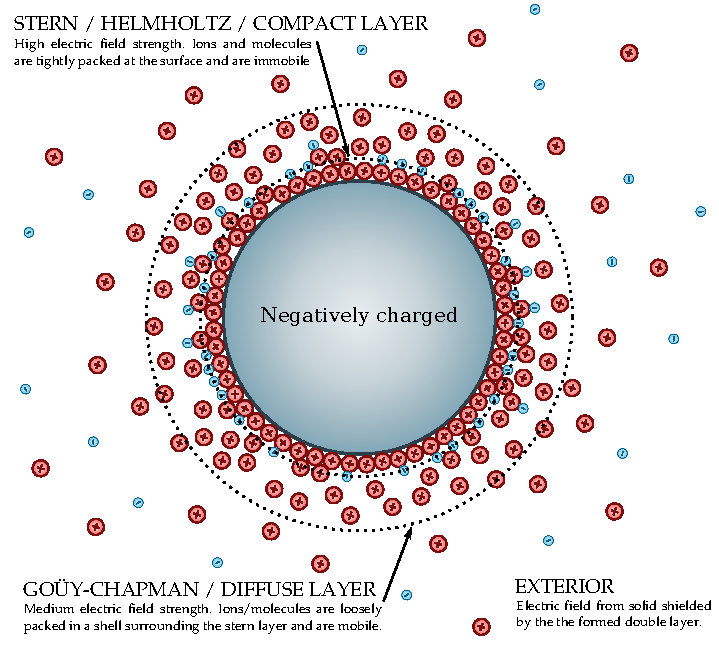
\includegraphics{content/introduction/graphics/doubleLayer_labelled.pdf}
    \end{center}
    \caption{Anatomy of the double layer}
    \label{fig:doubleLayer_anatomy}
\end{figure}

Double layers appear to varying degrees almost everywhere an electrolytic fluid and a solid are in contact. They are very small {Todo: quantify typical double layer sizes}, existing in the micro scale, and are responsible for a number of macro scale effects. Such effects are the stability of emulsions {Todo: find instances where double layers play a role}, the something else and even... They are a natural response when two systems of arrangement are brought to contact - fixed and fluid arrangements of charged particles.

\section{Physical Description}
    Double layer formation is the result of a liquid system responding to an imbalance of charge distribution. Atoms within a solid domain are static, they cannot repel each other or rearrange themselves. In a fluid the opposite is true, each freely moving charged entity will attempt to distance itself from others of like charge and move toward those of opposite charge. When these two domains are brought into contact with one another, the one whose elements are free to move (the liquid), moves to accommodate the imbalance in charge between the two domains. The effect of which is that an electrolytic liquid attracts atoms and molecules with a net opposite charge to the surface of the solid.

\subsection{Illustrated formation of a double layer}
    Figures \ref{fig:doubleLayer_set1} and \ref{fig:doubleLayer_set2} illustrate the formation of such a layer around a charged object that, for the sake of illustration, instantaneously appears in a settled electrolyte solution. In these figures, the spacing of depicted fluid elements do not represent the density of a liquid system and the smooth surface of the charged object in no way resembles the surface of a solid at the scale of individual atoms.

    The first set of images, figure \ref{fig:doubleLayer_set1}, depict charged elements in the fluid responding to the presence of the solid by aligning themselves with the induced field and migrating toward or away from the object. The second set of images, figure \ref{fig:doubleLayer_set2}, shows continued migration of charged particles and the formation of the Stern layer at the solid-liquid interface. Members of this layer are bound so strongly to the object that they are effectively immobile, i.e., they are adsorbed to the solid object. A substantial proportion of the initial electrical field from the solid is shielded by the Stern layer.

    Outside the Stern layer, as the field strength continues to diminish with increasing radial distance, ions and molecules are attracted with decreasing strength. This reduction in attraction forms a layer that is thicker than the stern layer and mobile; the ions are free to move locally within this secondary layer. This secondary layer is called the diffuse layer and it is convenient to visualise it as a fluffy cloud of charged particles attracted to, but not trapped upon, the thin Stern layer immediately adjacent to the surface.



    \begin{figure}
        \begin{center}
            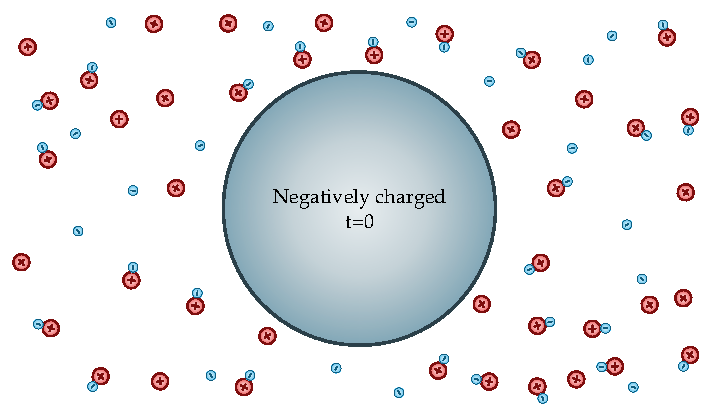
\includegraphics{content/introduction/graphics/doubleLayer_t0.pdf}
            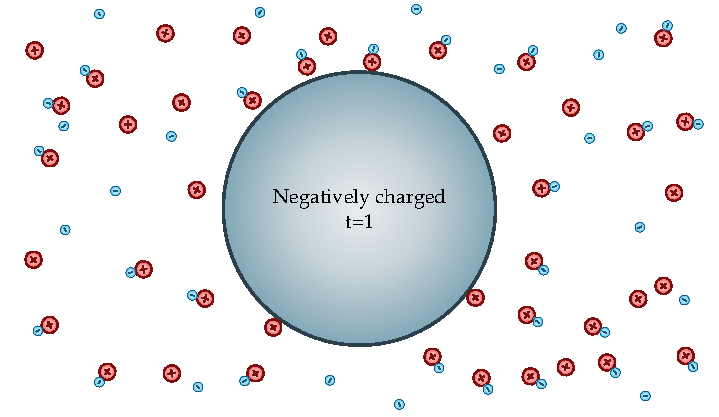
\includegraphics{content/introduction/graphics/doubleLayer_t1.pdf}
            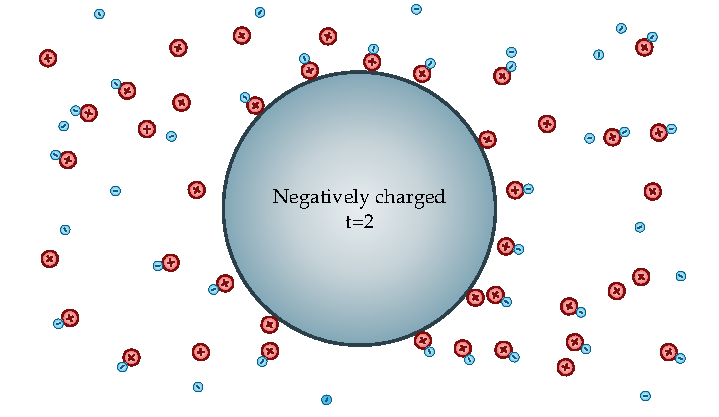
\includegraphics{content/introduction/graphics/doubleLayer_t2.pdf}
        \end{center}
        \caption{Creation of a double layer (time 0-2)}
        \label{fig:doubleLayer_set1}
    \end{figure}

    \begin{figure}
        \begin{center}
            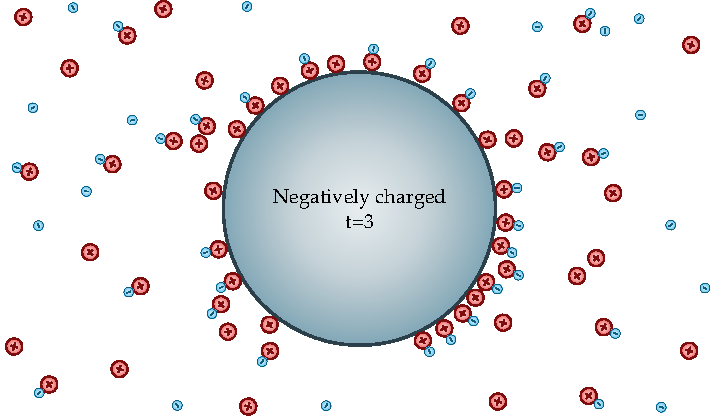
\includegraphics{content/introduction/graphics/doubleLayer_t3.pdf}
            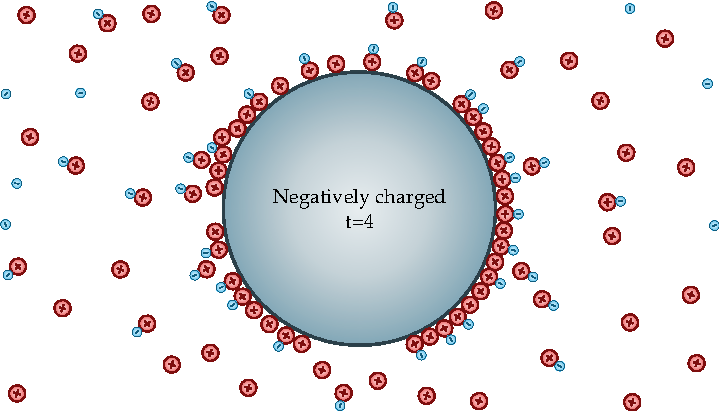
\includegraphics{content/introduction/graphics/doubleLayer_t4.pdf}
            %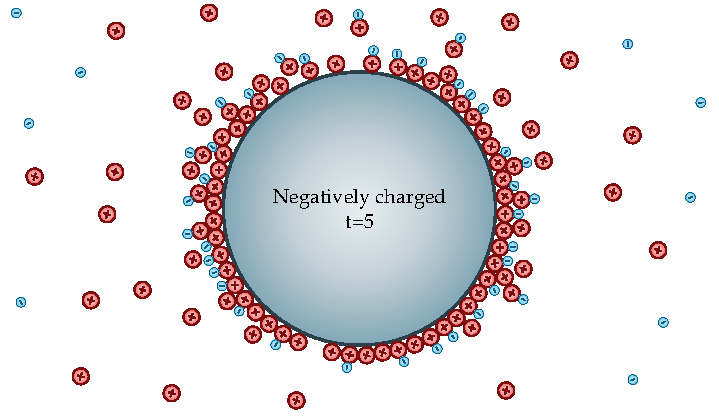
\includegraphics{content/introduction/graphics/doubleLayer_t5.pdf}
            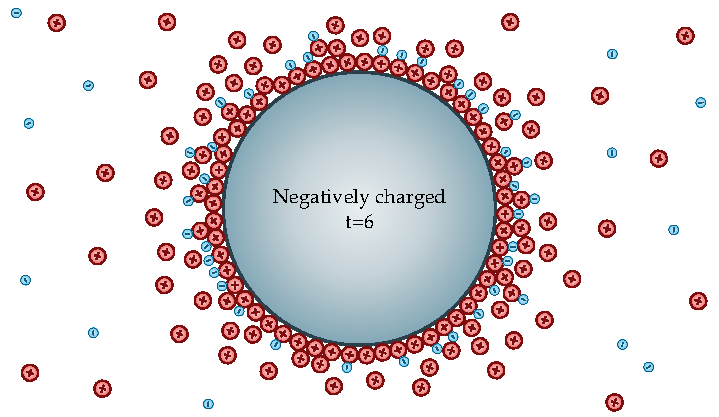
\includegraphics{content/introduction/graphics/doubleLayer_t6.pdf}
        \end{center}
        \caption{Creation of a double layer (time 3-6)}
        \label{fig:doubleLayer_set2}
    \end{figure}

\subsection{Criteria for formation}

    It is important to note that in order for a double layer to form, the liquid phase must contain ions, charged molecules, or polar molecules. This means of course that there are likely to be non-participating elements within the fluid, that is, elements not affected by the charge {Todo: check affected and effected} of surrounding elements.
    The reverse case is also true {Todo: is this correct?, I just made it up} where an electrolyte solution comes in contact with a electrically neutral and stable solid. Although this case is not as obvious as one may think. For example, placing pure water in a glass flask, it may be assumed, would not cause the formation of a double layer. Glassware in used throughout chemistry laboratories as it reacts with very little and pure water with no salt ions should be fairly stable. This is not the case however as glass in contact with water undergoes a process of deprotonation at the boundary. This deprotonation is where $H^{+}$ ions are torn from the surface of the glass and enter the liquid phase. As this happens, the surface of the glass is left negatively charged. Subsequently, a double layer is formed from polar water molecules and hydrated protons.


\section{Electrical Behaviour}

    \subsection{Capacitive Action}
    \subsection{Methods of Modelling}

